
\section{\label{sec:newtonsMethod}Metode Newton\index{metode Newton}\index{metode!Newton|see{metode Newton}}}

Pada bagian \ref{sec:fixedptOrder}, kita membahas sebagian kekurangan
iterasi titik tetap, tetapi menunda pembahasan mendalam tentang fungsi
misterius $f_{6}$ dari penyelidikan pencarian akar \vpageref{subsec:RootFindingInvestigation}.
Kini saatnya membahas $f_{6}$ secara lebih terperinci. Kita mulai
dengan beberapa perhitungan numerik. Ingat bahwa $f_{6}(x)=\frac{2x^{3}\text{\textminus}5x^{2}\text{\textminus}6}{3x^{2}\text{\textminus}10x+4}$
dan tetapkan $x_{0}=4.$ Dengan melanjutkan iterasi titik tetap,
\begin{eqnarray*}
x_{1}=f_{6}(x_{0}) & = & 3.5\\
x_{2}=f_{6}(x_{1}) & \approx & 3.217391304347826\\
x_{3}=f_{6}(x_{2}) & \approx & 3.072749058541597\\
x_{4}=f_{6}(x_{3}) & \approx & 3.013730618589344\\
x_{5}=f_{6}(x_{4}) & \approx & 3.000683798275568\\
x_{6}=f_{6}(x_{5}) & \approx & 3.000001860777997\\
x_{7}=f_{6}(x_{6}) & \approx & 3.000000000013848.
\end{eqnarray*}
Anda dapat melihat dua hal. Barisan $x_{0},x_{1},x_{2},\ldots$
\begin{enumerate}
\item konvergen ke (titik tetap) 3; dan
\item tampaknya kekonvergenannya kuadratik karena, sejak peralihan dari
$x_{4}$ ke $x_{5}$, jumlah angka signifikan kira-kira berlipat dua
pada setiap iterasi.
\end{enumerate}
Dalam analisis pada bagian \ref{sec:fixedptOrder} \vpageref{sec:fixedptOrder},
kita menemukan bahwa iterasi titik tetap konvergen secara kuadratik
(atau lebih cepat) hanya ketika turunan di titik tetap bernilai nol.
Pengamatan ini semestinya membuat Anda menduga bahwa $f_{6}'(3)=0$.
Mari kita periksa. Pertama, turunannya adalah $f_{6}'(x)=\frac{6x^{4}\text{\textminus}40x^{3}+74x^{2}\text{\textminus}4x\text{\textminus}60}{(3x^{2}\text{\textminus}10x+4)^{2}}$
(Anda sebaiknya memverifikasi ini). Dengan mengevaluasi pembilang
di titik tetap, $x=3$, kita memperoleh $6(3)^{4}-40(3)^{3}+74(3)^{2}-4(3)-60=486-1080+666-12-60=0$.
Jadi, kita memperoleh kekonvergenan menuju titik tetap tempat turunan
fungsi bernilai nol, dan memang kekonvergenannya kuadratik.

Dengan $x_{0}=2$ sebagai nilai awal, iterasi titik tetap pada $f_{6}$
konvergen ke $1+\sqrt{3}$, sedangkan dengan $x_{0}=-1$ sebagai nilai
awal, iterasi titik tetap konvergen ke $1-\sqrt{3}$. Anda seharusnya
dapat memverifikasi hal ini dari diagram kekonvergenan pada Gambar
\ref{fig:SixConvergenceDiagrams} atau dengan menghitung sendiri beberapa
iterasi pertama untuk masing-masing kasus. Yang tidak ditunjukkan
oleh diagram kekonvergenan adalah laju kekonvergenannya. Untuk itu,
Anda perlu melihat hasil-hasil iterasinya. Silakan lakukan. Apakah
kekonvergenannya juga tampak kuadratik dalam kasus-kasus ini? Jawaban
\vpageref{que:quadraticConvergence}.

Dari diagram kekonvergenan, kita melihat bahwa iterasi titik tetap
akan konvergen untuk hampir semua nilai awal, dan ketiga titik tetap
dapat dihampiri dengan iterasi titik tetap. Selain itu, dari perhitungan
kita, tampaknya kekonvergenannya kuadratik untuk ketiganya. Sulit
mengharapkan lebih banyak dari suatu fungsi. Kekonvergenan yang cepat
menuju titik tetap mana pun! Jadi, dari mana $f_{6}$ berasal?

Misalkan $g(x)$ terdiferensialkan dan $g(\hat{x})=0$, sehingga $g$
memiliki akar di $\hat{x}$. Tinjau $f(x)=x-\frac{g(x)}{g'(x)}$.
$\hat{x}$ merupakan titik tetap $f$ selama $g'(\hat{x})\neq0$:
\[
f(\hat{x})=\hat{x}-\frac{g(\hat{x})}{g'(\hat{x})}=\hat{x}-\frac{0}{g'(\hat{x})}=\hat{x}.
\]
Selain itu, selama $g$ memiliki turunan kedua di sekitar $\hat{x}$,
\begin{eqnarray*}
f'(\hat{x}) & = & 1-\frac{g'(\hat{x})\cdot g'(\hat{x})-g(\hat{x})g''(\hat{x})}{g'(\hat{x})\cdot g'(\hat{x})}\\
 & = & 1-1+\frac{0\cdot g''(\hat{x})}{g'(\hat{x})\cdot g'(\hat{x})}\\
 & = & 0.
\end{eqnarray*}
Dari perhitungan ini, kita menyimpulkan bahwa jika $g(x)$ terdiferensialkan
dua kali, $g(\hat{x})=0$ dan $g'(\hat{x})\neq0$, maka iterasi titik
tetap untuk $f(x)$ dengan nilai awal di suatu lingkungan $\hat{x}$
akan konvergen secara kuadratik ke $\hat{x}$. Sungguh cara yang hebat
untuk mengubah masalah pencarian akar menjadi masalah titik tetap!

Sekarang saat yang tepat untuk mengingat bahwa $f_{6}$ hanyalah salah
satu dari 6 fungsi kandidat yang dirancang untuk mencari akar dari
$g(x)=-x^{3}+5x^{2}-4x-6$ dengan iterasi titik tetap. Memang, $g'(x)=-3x^{2}+10x-4$
dan 
\begin{eqnarray*}
x-\frac{g(x)}{g'(x)} & = & x-\frac{-x^{3}+5x^{2}-4x-6}{-3x^{2}+10x-4}\\
 & = & \frac{2x^{3}\text{\textminus}5x^{2}\text{\textminus}6}{3x^{2}\text{\textminus}10x+4}\\
 & = & f_{6}(x).
\end{eqnarray*}
Penggunaan iterasi titik tetap pada $f_{6}(x)=x-\frac{g(x)}{g'(x)}$
untuk mencari akar $g(x)$, seperti yang dilakukan di sini, disebut
\index{metode Newton} metode Newton.

\subsection{Penurunan Geometris Metode Newton}

\noindent Gambar berikut menunjukkan cara menghitung dua iterasi pertama
metode Newton pada $g(x)=-x^{3}+5x^{2}-4x-6$ dengan nilai awal $x_{0}=-2.5$
secara geometris.

\begin{center}
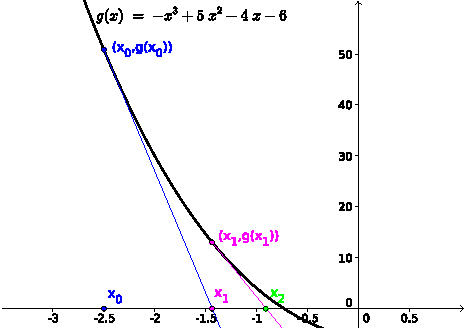
\includegraphics{figures/roots-newton1}\label{img:newtonsMethod}
\par\end{center}

\noindent Untuk menghitung $x_{1}$, tarik garis singgung pada $g$
di $(x_{0},g(x_{0}))$; perpotongan garis ini dengan sumbu $x$ adalah
$x_{1}$. Demikian pula, tarik garis singgung pada $g$ di $(x_{1},g(x_{1}))$;
perpotongan garis ini dengan sumbu $x$ adalah $x_{2}$. Demikian
seterusnya. Sebagai contoh, $(x_{0},g(x_{0}))=(-2.5,50.875)$ dan
$g'(x_{0})=g'(-2.5)=-47.75$. Oleh karena itu, ``perubahan vertikal''
($0-50.875$) dibagi ``perubahan horizontal'' ($x_{1}+2.5$) antara
$(-2.5,50.875)$ dan $(x_{1},0)$ harus sama dengan $-47.75$. Dengan
demikian, kita memperoleh $\frac{-50.875}{x_{1}+2.5}=-47.75$ sehingga
\[
x_{1}=\frac{-50.875}{-47.75}-2.5\approx-1.43455497382199.
\]
Dalam simbol, ``perubahan vertikal'' ($-g(x_{0})$) dibagi ``perubahan
horizontal'' ($x_{1}-x_{0})$ harus sama dengan $g'(x_{0})$. Dengan
kata lain,
\begin{eqnarray*}
\frac{-g(x_{0})}{x_{1}-x_{0}} & = & g'(x_{0})\Rightarrow\\
\frac{-g(x_{0})}{g'(x_{0})} & = & x_{1}-x_{0}\Rightarrow\\
x_{1} & = & x_{0}-\frac{g(x_{0})}{g'(x_{0})}.
\end{eqnarray*}
Perhitungan serupa menunjukkan $x_{2}=x_{1}-\frac{g(x_{1})}{g'(x_{1})}$,
dan secara lebih umum $x_{n+1}=x_{n}-\frac{g(x_{n})}{g'(x_{n})}$.
Relasi rekurensi ini menjelaskan metode Newton---yakni mengiterasikan
fungsi $f(x)=x-\frac{g(x)}{g'(x)}$.

\subsection{Metode Newton (kode semu)\index{metode Newton!kode semu}}

Tidak seperti pada metode Steffensen, penyebut dalam metode Newton
tidak diharapkan mendekati nol ketika hasil-hasil iterasinya konvergen;
karena itu, secara umum kestabilan perhitungan jauh lebih jarang bermasalah
dan tidak dilakukan pemeriksaan perantara sebelum menghitung satu
iterasi dari iterasi sebelumnya.

\begin{pseudocode} 
\begin{description}
\item [{Asumsi:}] $g$ terdiferensialkan dua kali. $g$ memiliki akar di
$\hat{x}$. $x_{0}$ berada dalam lingkungan $(\hat{x}-\delta,\hat{x}+\delta)$
tempat nilai mutlak $f'(x)=1-\frac{g'(x)\cdot g'(x)-g(x)g''(x)}{g'(x)\cdot g'(x)}$
kurang dari satu.
\item [{Masukan:}] Nilai awal $x_{0}$; fungsi $g$ beserta turunannya
$g'$; akurasi yang diinginkan $tol$; jumlah iterasi maksimum $N$.
\item [{Langkah~1:}] Untuk $j=1\ldots N$ lakukan Langkah 2--4:

\begin{description}
\item [{Langkah~2:}] Tetapkan $x=x_{0}-\frac{g(x_{0})}{g'(x_{0})}$;
\item [{Langkah~3:}] Jika $|x-x_{0}|\leq tol$ maka kembalikan $x$;
\item [{Langkah~4:}] Tetapkan $x_{0}=x$;
\end{description}
\item [{Langkah~5:}] Cetak ``Metode gagal. Jumlah iterasi maksimum terlampaui.''
\item [{Keluaran:}] Hampiran $x$ di dekat titik tetap eksak, atau pesan
kegagalan.
\end{description}
\end{pseudocode}  

\subsection{Metode Sekan\index{metode sekan}\index{metode!sekan|see{metode sekan}}}

Kelemahan terbesar metode Newton adalah keharusan untuk mengetahui
$g'$ dan menggunakannya dalam perhitungan. Namun, turunan tidak selalu
tersedia, mudah ditangani, atau bahkan diketahui. Dalam kasus seperti
itu, lebih baik menggunakan metode Steffensen atau metode sekan. Metode
sekan diturunkan dengan mengganti $g'$ dalam metode Newton dengan
hasil bagi selisih. Agar penggantian ini masuk akal, kita perlu menyatakan
kembali metode Newton dalam bentuk $x_{n}$. Dalam metode Newton,
kita mengiterasikan $f(x)=x-\frac{g(x)}{g'(x)}$ sehingga $x_{n+1}=x_{n}-\frac{g(x_{n})}{g'(x_{n})}$.

Sekarang, misalkan Anda memiliki fungsi $g$ dan suatu hasil iterasi
$x_{n-1}$. Informasi ini cukup untuk menentukan satu titik pada grafik
$g$, yaitu $(x_{n-1},g(x_{n-1}))$. Namun, kita memerlukan satu titik
lagi untuk membentuk hasil bagi selisih (kemiringan garis yang melalui
dua titik). Maka, misalkan kita memiliki nilai kedua, $x_{n}$, yang
dekat dengan $x_{n-1}$. Maka, $\frac{g(x_{n})-g(x_{n-1})}{x_{n}-x_{n-1}}\approx g'(x_{n})$
sehingga kita dapat mengganti $\frac{g(x_{n})-g(x_{n-1})}{x_{n}-x_{n-1}}$
sebagai pengganti $g'(x_{n})$ dalam metode Newton. Penggantian ini
menghasilkan \index{metode sekan} metode sekan, $x_{n+1}=x_{n}-g(x_{n})/\left(\frac{g(x_{n})-g(x_{n-1})}{x_{n}-x_{n-1}}\right)$,
yang dapat disederhanakan menjadi
\begin{equation}
x_{n+1}=x_{n}-g(x_{n})\frac{x_{n}-x_{n-1}}{g(x_{n})-g(x_{n-1})}.\label{eq:secantMethod}
\end{equation}
Secara geometris, dapatkah Anda melihat cara kerja metode ini? Jawaban
\vpageref{que:secantMethodGeometrically}. Perhatikan bahwa ini tidak
sepenuhnya merupakan skema iterasi titik tetap. Setiap iterasi bergantung
pada \textit{dua} nilai sebelumnya, bukan satu. Analisis yang telah
kita lakukan sejauh ini tidak berlaku, tetapi ada harapan bahwa kekonvergenannya
akan cepat karena metode ini merupakan hampiran yang wajar terhadap
metode Newton di dekat suatu akar, dengan asumsi $g$ terdiferensialkan
di sekitar akar tersebut. Tabel 
\begin{table}
\hrule 

\caption{\label{tab:secantDemo} Metode sekan yang diterapkan pada $g(x)=-x^{3}+5x^{2}-4x-6$
dengan $x_{0}=5$ dan $x_{1}=x_{0}+g(x_{0})=-21$.}

\centering{}\medskip{}
\begin{tabular}{ccc}
$n$ & $x_{n}$ & $|3-x_{n}|$\tabularnewline
\hline 
0 & $5$ & $2(10)^{0}$\tabularnewline
1 & $-21$ & $2.4(10)^{1}$\tabularnewline
2 & $4.9415730337078$ & $1.941(10)^{0}$\tabularnewline
3 & $4.8869924815972$ & $1.886(10)^{0}$\tabularnewline
4 & $4.0502898397912$ & $1.050(10)^{0}$\tabularnewline
5 & $3.7088949488497$ & $7.088(10)^{-1}$\tabularnewline
6 & $3.412824115541$ & $4.128(10)^{-1}$\tabularnewline
7 & $3.232292913133$ & $2.322(10)^{-1}$\tabularnewline
8 & $3.1141957095727$ & $1.141(10)^{-1}$\tabularnewline
9 & $3.0465011115969$ & $4.650(10)^{-2}$\tabularnewline
10 & $3.0132833760752$ & $1.328(10)^{-2}$\tabularnewline
11 & $3.0020189248976$ & $2.018(10)^{-3}$\tabularnewline
12 & $3.0001014520965$ & $1.014(10)^{-4}$\tabularnewline
13 & $3.0000008128334$ & $8.128(10)^{-7}$\tabularnewline
14 & $3.0000000003297$ & $3.297(10)^{-10}$\tabularnewline
\end{tabular}\medskip{}
\hrule 
\end{table}
\ref{tab:secantDemo} memberikan bukti bahwa metode sekan memang konvergen
dengan cepat. Dalam kasus khusus $g(x)=-x^{3}+5x^{2}-4x-6$ dengan
$x_{0}=5$ dan $x_{1}=x_{0}+g(x_{0})=-21$, diperlukan beberapa saat
sampai perilakunya stabil, tetapi setelah kira-kira 8 iterasi pertama,
kekonvergenannya sangat cepat. Tidak sepenuhnya kuadratik, tetapi
jelas superlinear.

\begin{digression}{Metode sekan konvergen dengan orde $\frac{1+\sqrt{5}}{2}$.}

\noindent\index{metode sekan!analisis}Misalkan $g$ adalah fungsi
dengan akar $\hat{x}$, $g'(\hat{x})\neq0$, $g''(\hat{x})\neq0$,
dan $g'''(x)$ ada di suatu lingkungan $\hat{x}$. Misalkan $x_{0},x_{1},x_{2},\ldots$
adalah barisan yang diperoleh dari metode sekan ($x_{n+1}=x_{n}-g(x_{n})\frac{x_{n}-x_{n-1}}{g(x_{n})-g(x_{n-1})}$
untuk semua $k\geq2$) sedemikian sehingga ${\displaystyle \lim_{k\to\infty}x_{k}=\hat{x}}$.
Definisikan $e_{n}=x_{n}-\hat{x}$ sehingga $x_{n}=\hat{x}+e_{n}$.
Dengan melakukan substitusi ini ke dalam \ref{eq:secantMethod} kita
memperoleh 
\begin{equation}
e_{n+1}=e_{n}-g(\hat{x}+e_{n})\frac{e_{n}-e_{n-1}}{g(\hat{x}+e_{n})-g(\hat{x}+e_{n-1})}.\label{eq:secantOrderPart1}
\end{equation}
Teorema Taylor memberikan $g(\hat{x}+e_{k})=g(\hat{x})+e_{k}g'(\hat{x})+\frac{1}{2}e_{k}^{2}g''(\hat{x})+O(e_{k}^{3})$.
Dengan memperhatikan bahwa $g(\hat{x})=0$ dan mensubstitusikannya
ke dalam \ref{eq:secantOrderPart1},
\begin{eqnarray}
e_{n+1} & = & e_{n}-(e_{n}-e_{n-1})\frac{e_{n}g'(\hat{x})+\frac{1}{2}e_{n}^{2}g''(\hat{x})+O(e_{n}^{3})}{(e_{n}-e_{n-1})g'(\hat{x})+\frac{1}{2}(e_{n}^{2}-e_{n-1}^{2})g''(\hat{x})+O(e_{n-1}^{3})}\nonumber \\
 & = & e_{n}-\frac{e_{n}+\frac{e_{n}^{2}g''(\hat{x})}{2g'(\hat{x})}+O(e_{n}^{3})}{1+\frac{(e_{n}+e_{n-1})g''(\hat{x})}{2g'(\hat{x})}+\frac{O(e_{n-1}^{3})}{(e_{n}-e_{n-1})}}\nonumber \\
 & = & \frac{e_{n}\left(1+\frac{(e_{n}+e_{n-1})g''(\hat{x})}{2g'(\hat{x})}+\frac{O(e_{n-1}^{3})}{(e_{n}-e_{n-1})}\right)-\left(e_{n}+\frac{e_{n}^{2}g''(\hat{x})}{2g'(\hat{x})}+O(e_{n}^{3})\right)}{1+\frac{(e_{n}+e_{n-1})g''(\hat{x})}{2g'(\hat{x})}+\frac{O(e_{n-1}^{3})}{(e_{n}-e_{n-1})}}\nonumber \\
 & = & \frac{e_{n}e_{n-1}\frac{g''(\hat{x})}{2g'(\hat{x})}+\frac{e_{n}}{e_{n}-e_{n-1}}O(e_{n-1}^{3})+O(e_{n}^{3})}{1+\frac{(e_{n}+e_{n-1})g''(\hat{x})}{2g'(\hat{x})}+\frac{O(e_{n-1}^{3})}{(e_{n}-e_{n-1})}}.\label{eq:secantOrderPart2}
\end{eqnarray}
Dengan menggunakan persamaan \ref{eq:secantOrderPart2} untuk mencari
nilai $\alpha$ yang memenuhi $\lim_{n\to\infty}\frac{|\hat{x}-x_{n+1}|}{|\hat{x}-x_{n}|^{\alpha}}=\lambda\neq0$,
kita memperoleh
\begin{eqnarray*}
\lim_{n\to\infty}\frac{|\hat{x}-x_{n+1}|}{|\hat{x}-x_{n}|^{\alpha}} & = & \lim_{n\to\infty}\frac{|e_{n+1}|}{|e_{n}|^{\alpha}}\\
 & = & \lim_{n\to\infty}\left|\frac{e_{n}^{1-\alpha}e_{n-1}\frac{g''(\hat{x})}{2g'(\hat{x})}+\frac{e_{n}^{1-\alpha}}{e_{n}-e_{n-1}}O(e_{n-1}^{3})+O(e_{n}^{3-\alpha})}{1+\frac{(e_{n}+e_{n-1})g''(\hat{x})}{2g'(\hat{x})}+\frac{O(e_{n-1}^{3})}{(e_{n}-e_{n-1})}}\right|\\
 & = & \lambda\neq0.
\end{eqnarray*}
Namun, $\lim_{n\to\infty}e_{n}=\lim_{n\to\infty}e_{n-1}=0$. Oleh
karena itu, $\lim_{n\to\infty}e_{n}^{1-\alpha}e_{n-1}$ tidak boleh
bernilai 0 ataupun divergen, sebab jika demikian, $\lim_{n\to\infty}\frac{|\hat{x}-x_{n+1}|}{|\hat{x}-x_{n}|^{\alpha}}$
masing-masing akan bernilai 0 atau divergen. Akibatnya, terdapat konstanta
positif $C$ sedemikian sehingga $\lim_{n\to\infty}|e_{n}^{1-\alpha}e_{n-1}|=\lim_{n\to\infty}|e_{n+1}^{1-\alpha}e_{n}|=C\Rightarrow\lim_{n\to\infty}|e_{n+1}e_{n}^{1/(1-\alpha)}|=C^{1/(1-\alpha)}$.
Sekarang kita memperoleh 
\[
\lim_{n\to\infty}\frac{|e_{n+1}|}{|e_{n}|^{\alpha}}=\lambda\neq0\mbox{ dan }\lim_{n\to\infty}\frac{|e_{n+1}|}{|e_{n}|^{1/(\alpha-1)}}=C^{1/(1-\alpha)}\neq0.
\]
Karena orde kekonvergenan suatu barisan bersifat unik (Latihan \ref{enu:orderOfConvergenceIsUnique}
pada bagian \ref{sec:Speed}), haruslah $\alpha=1/(\alpha-1)$ atau
$\alpha^{2}-\alpha-1=0$. Rumus kuadrat memberikan hasil yang diinginkan.

\end{digression}

Sejauh ini kita baru menerapkan metode Newton dan metode sekan pada
polinom kubik $g(x)=-x^{3}+5x^{2}-4x-6$, suatu pekerjaan yang sebenarnya
tidak diperlukan. Teorema akar rasional, alat dasar dalam prakalkulus,
akan memungkinkan Anda memperoleh akar-akarnya secara eksak. Teorema
tersebut meminta Anda memeriksa $\pm1,\pm2,\pm3,$ dan $\pm6$ sebagai
akar-akar yang mungkin dari $g$. Dengan asumsi bahwa Anda melakukan
pemeriksaan menggunakan pembagian sintetis, perhitungan Anda mungkin
tampak seperti ini:\label{syntheticDivisionExample}

\begin{center}
\begin{tabular}{ccccc}
\multicolumn{1}{c|}{$3$} & $-1$ & $5$ & $-4$ & $-6$\tabularnewline
\cline{1-1}
 &  & $-3$ & $6$ & $6$\tabularnewline
\hline 
 & $-1$ & $2$ & \multicolumn{1}{c|}{$2$} & \multicolumn{1}{c|}{$0$}\tabularnewline
\cline{5-5}
\end{tabular}
\par\end{center}

\noindent yang berarti $g(x)=(x-3)(-x^{2}+2x+2)$. Dua akar lainnya
kemudian diperoleh dengan menerapkan rumus kuadrat pada $-x^{2}+2x+2$
dan hasilnya adalah $\frac{-2\pm\sqrt{4+8}}{-2}=1\pm\sqrt{3}$.

\noindent\begin{digression}{Menyelesaikan persamaan kubik}  

\noindent Akar-akar persamaan kuadrat $ax^{2}+bx+c=0$ diberikan oleh
rumus kuadrat yang sudah dikenal luas. Yang kurang dikenal, dan jauh
lebih rumit, adalah rumus untuk memperoleh akar-akar \index{rumus kubik}
persamaan kubik $ax^{3}+bx^{2}+cx+d=0$. Salah satu metode penyelesaiannya
adalah sebagai berikut. Pertama, kita tetapkan
\begin{eqnarray*}
p & = & \frac{3ac-b^{2}}{3a^{2}}\qquad\mbox{dan}\\
q & = & \frac{2b^{3}-9abc+27a^{2}d}{27a^{3}}.
\end{eqnarray*}
Kemudian kita tetapkan 
\[
w^{3}=-\frac{q}{2}-\sqrt{\frac{q^{2}}{4}+\frac{p^{3}}{27}}.
\]
Ketiga, kita tetapkan $w_{1},w_{2},$ dan $w_{3}$ sebagai tiga nilai
(kompleks) yang mungkin bagi $w$. Terakhir, ketiga penyelesaian $ax^{3}+bx^{2}+cx+d=0$
adalah 
\[
x_{i}=w_{i}-\frac{p}{3w_{i}}-\frac{b}{3a},\quad i=1,2,3.
\]
Ini pada dasarnya adalah metode \index{Cardano!rumus kubik} Cardano,
yang diterbitkan pada abad ke-$16$!

Sebagai contoh, untuk menyelesaikan persamaan $-x^{3}+5x^{2}-4x-6=0$,
kita mulai dengan
\begin{eqnarray*}
p & = & \frac{3(-1)(-4)-5^{2}}{3(-1)^{2}}=-\frac{13}{3}\qquad\mbox{dan}\\
q & = & \frac{2\cdot5^{3}-9(-1)(5)(-4)+27(-1)^{2}(-6)}{27(-1)^{3}}=\frac{92}{27}.
\end{eqnarray*}
Kemudian
\begin{eqnarray*}
w^{3} & = & -\frac{92}{2\cdot27}-\sqrt{\frac{92^{2}}{4\cdot27^{2}}-\frac{13^{3}}{27^{2}}}\\
 & = & -\frac{46}{27}-\frac{\sqrt{92^{2}-4\cdot13^{3}}}{54}\\
 & = & -\frac{46}{27}-\frac{\sqrt{-324}}{54}\\
 & = & -\frac{46}{27}-\frac{i}{3}.
\end{eqnarray*}
Dalam bentuk polar, $w^{3}=\frac{13\sqrt{13}}{27}e^{i(\tan^{-1}(9/46)-\pi)}$
sehingga kita dapat menetapkan $w_{1}=\frac{\sqrt{13}}{3}e^{i(\tan^{-1}(9/46)-\pi)/3}$,
salah satu akar pangkat tiga dari $w^{3}$. Sayangnya, menentukan
sudut $(\tan^{-1}(9/46)-\pi)/3$ secara eksak setara dengan menyelesaikan
persamaan kubik! Namun, dengan bantuan kalkulator, kita dapat memperoleh
hampiran $\text{\textminus}0.982793723247329$, yang pada akhirnya
cukup baik. Jadi, bagian real dari $w_{1}$ kira-kira $\frac{\sqrt{13}}{3}\cos(\text{\textminus}0.982793723247329)\approx.6666666666666667$
dan bagian imajinernya kira-kira $\frac{\sqrt{13}}{3}\sin(\text{\textminus}0.982793723247329)\approx-1$.
$w_{1}$ sangat dekat dengan $\frac{2}{3}-i$. Dan kita dapat memeriksa,
$\left(\frac{2}{3}-i\right)^{3}=\left(\frac{2}{3}\right)^{3}+3\left(\frac{2}{3}\right)^{2}(-i)+3\cdot\frac{2}{3}(-i)^{2}+(-i)^{3}=\frac{8}{27}-\frac{12}{9}i-2+i=-\frac{46}{27}-\frac{1}{3}i$.
Oleh karena itu, $w_{1}=\frac{2}{3}-i$ dan kita tetapkan $w_{2}=\left(\frac{2}{3}-i\right)\left(-\frac{1}{2}+\frac{\sqrt{3}}{2}i\right)=\frac{3\sqrt{3}-2}{6}+\frac{3+2\sqrt{3}}{6}i$
serta $w_{3}=\left(\frac{2}{3}-i\right)\left(-\frac{1}{2}-\frac{\sqrt{3}}{2}i\right)=\frac{-3\sqrt{3}-2}{6}+\frac{3-2\sqrt{3}}{6}i$.
Terakhir,
\begin{eqnarray*}
x_{1} & = & w_{1}+\frac{13}{9w_{1}}+\frac{5}{3}=w_{1}+\frac{13\overline{w_{1}}}{9|w_{1}|^{2}}+\frac{5}{3}=w_{1}+\overline{w_{1}}+\frac{5}{3}=3\\
x_{2} & = & w_{2}+\frac{13}{9w_{2}}+\frac{5}{3}=w_{2}+\frac{13\overline{w_{2}}}{9|w_{2}|^{2}}+\frac{5}{3}=w_{2}+\overline{w_{2}}+\frac{5}{3}=\sqrt{3}+1\\
x_{3} & = & w_{3}+\frac{13}{9w_{3}}+\frac{5}{3}=w_{3}+\frac{13\overline{w_{3}}}{9|w_{3}|^{2}}+\frac{5}{3}=w_{3}+\overline{w_{3}}+\frac{5}{3}=-\sqrt{3}+1
\end{eqnarray*}

\noindent\end{digression}

Untuk sebuah persamaan yang kemungkinan besar belum pernah Anda jumpai
dalam prakalkulus, bahkan dalam kalkulus sekalipun, tinjau \label{interestingNewton}
\[
x-e^{x}\cos\sqrt{e^{2x}-x^{2}}=0.
\]
Anda mungkin mencoba menyelesaikan persamaan ini secara eksak dengan
pensil dan kertas, tetapi akan segera menemui jalan buntu. Persamaan
ini tidak dapat diselesaikan secara eksplisit. Yang paling dapat Anda
harapkan adalah menghampiri penyelesaiannya dengan metode numerik.
Untuk memperoleh gambaran tentang apa yang akan kita hadapi, lihat
grafik $x-e^{x}\cos\sqrt{e^{2x}-x^{2}}$ pada Gambar 
\begin{figure}

\caption{\label{fig:rootFindingExample}Grafik $x-e^{x}\cos\sqrt{e^{2x}-x^{2}}$
memotong sumbu $x$ tak berhingga kali.}

\centering{}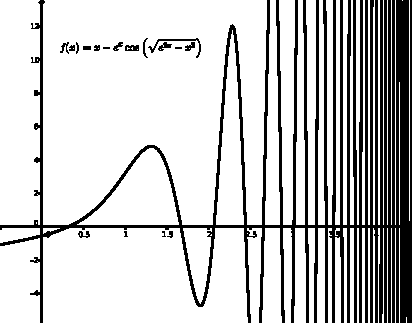
\includegraphics{figures/roots-newton2}
\end{figure}
 \ref{fig:rootFindingExample}. Fungsi ini berosilasi secara liar,
dan osilasinya semakin liar ketika $x$ bertambah. Grafik memotong
sumbu $x$ sebanyak 29 kali pada interval dari $0$ hingga $4.5$
sehingga mempunyai 29 akar di sana! Akar-akarnya adalah
\[
\begin{gathered}.3181315052047641,\ 1.668024051576096,\ 2.062277729598284,\\
2.439940377216816,\ 2.653191974038697,\ldots
\end{gathered}
\]
dan dapat ditemukan dengan metode Newton menggunakan nilai awal $0,1.5,2,2.4,2.6,\ldots$.
Dapatkah Anda menemukan akar berikutnya? Jawaban \vpageref{que:nextRoot}.

\subsection{Metode Sekan (kode semu)\index{metode sekan!kode semu}}

Implementasi langsung metode sekan dapat dengan mudah menjadi tidak
efisien karena banyaknya kemunculan $g$ dalam rumus (\ref{eq:secantMethod}).
Kode semu di bawah ini sangat berhati-hati agar tidak menghitung setiap
nilai $g$ lebih dari sekali. Jika kode itu tampak lebih rumit daripada
yang diperlukan, kemungkinan inilah sumber kerumitannya.

\begin{pseudocode} 
\begin{description}
\item [{Asumsi:}] $g$ mempunyai akar di $\hat{x}$. $g$ terdiferensialkan
dalam suatu lingkungan $\hat{x}$. $x_{0}$ dan $x_{1}$ cukup dekat
dengan $\hat{x}$.
\item [{Masukan:}] Nilai awal $x_{0}$ dan $x_{1}$; fungsi $g$; akurasi
yang diinginkan $tol$; jumlah maksimum iterasi $N$.
\item [{Langkah~1:}] Tetapkan $y_{0}=g(x_{0})$; $y_{1}=g(x_{1})$
\item [{Langkah~2:}] Untuk $j=1\ldots N$ lakukan Langkah 3--5:

\begin{description}
\item [{Langkah~3:}] Tetapkan $x=x_{1}-y_{1}\frac{x_{1}-x_{0}}{y_{1}-y_{0}}$;
\item [{Langkah~4:}] Jika $|x-x_{1}|\leq tol$ maka kembalikan $x$;
\item [{Langkah~5:}] Tetapkan $x_{0}=x_{1}$; $y_{0}=y_{1}$; $x_{1}=x$;
$y_{1}=g(x_{1})$
\end{description}
\item [{Langkah~6:}] Cetak ``Metode gagal. Jumlah maksimum iterasi terlampaui.''
\item [{Keluaran:}] Hampiran $x$ yang mendekati akar eksak, atau pesan
kegagalan.
\end{description}
\end{pseudocode}  

\subsection{Metode Sekan dengan Satu Nilai Awal (kode semu) \index{metode sekan dengan satu nilai awal}\index{metode!sekan dengan satu nilai awal|see{metode sekan dengan satu nilai awal}}\index{metode sekan dengan satu nilai awal!kode semu}}

Kelemahan terbesar metode sekan adalah keharusan adanya dua nilai
awal. Keduanya harus berdekatan, tetapi seberapa dekat, dan bagaimana
Anda menentukannya? Pertanyaan-pertanyaan ini sulit, dan jawaban paling
sederhana sekalipun tetap rumit. Salah satu pendekatan yang masuk
akal ialah menetapkan $x_{1}=x_{0}+g(x_{0})$. Dengan asumsi $x_{0}$
dekat dengan suatu akar, $g(x_{0})$ akan kecil, sehingga $x_{1}$
akan dekat dengan $x_{0}$. Pendekatan ini membebaskan pengguna dari
beban memilih nilai awal kedua. Ada kalanya pemilihan otomatis semacam
itu tidak diinginkan, sehingga metode sekan dengan dua nilai awal
dan metode sekan dengan satu nilai awal sama-sama berguna. Metode
sekan dengan satu nilai awal hanya bekerja dengan baik jika hampiran
awalnya baik.

\begin{pseudocode} 
\begin{description}
\item [{Asumsi:}] $g$ mempunyai akar di $\hat{x}$. $g$ terdiferensialkan
dalam suatu lingkungan $\hat{x}$. $x_{0}$ cukup dekat dengan $\hat{x}$.
\item [{Masukan:}] Nilai awal $x_{0}$; fungsi $g$; akurasi yang diinginkan
$tol$; jumlah maksimum iterasi $N$.
\item [{Langkah~1:}] Tetapkan $y_{0}=g(x_{0})$; $x_{1}=x_{0}+y_{0}$;
$y_{1}=g(x_{1})$
\item [{Langkah~2:}] Untuk $j=1\ldots N$ lakukan Langkah 3--5:

\begin{description}
\item [{Langkah~3:}] Tetapkan $x=x_{1}-y_{1}\frac{x_{1}-x_{0}}{y_{1}-y_{0}}$;
\item [{Langkah~4:}] Jika $|x-x_{1}|\leq tol$ maka kembalikan $x$;
\item [{Langkah~5:}] Tetapkan $x_{0}=x_{1}$; $y_{0}=y_{1}$; $x_{1}=x$;
$y_{1}=g(x_{1})$
\end{description}
\item [{Langkah~6:}] Cetak ``Metode gagal. Jumlah iterasi maksimum terlampaui.''
\item [{Keluaran:}] Hampiran $x$ di dekat akar eksak, atau pesan kegagalan.
\end{description}
\end{pseudocode}  

\subsection{Konsep Utama}
\begin{description}
\item [{Teorema~Akar~Rasional:}] \index{Teorema!Akar Rasional} Jika
polinom $p(x)=a_{0}+a_{1}x+\cdots+a_{k}x^{k}$ memiliki koefisien
rasional, maka setiap akar rasional dari $p$ termasuk dalam himpunan
$\left\{ \frac{n}{d}:n\mbox{ merupakan faktor dari }a_{0}\mbox{ dan }d\mbox{ merupakan faktor dari }a_{k}\right\} $.
\item [{Pembagian~sintetis:}] \index{pembagian!sintetis} Metode untuk
menghitung hasil bagi suatu polinom oleh suatu monomial. Contoh \vpageref{syntheticDivisionExample}.
\item [{Metode~Newton:}] \index{metode Newton} Metode pencarian akar
yang umumnya berkonvergensi ke suatu akar dari $g(x)$ secara kuadratik,
tetapi memerlukan penggunaan turunan. Dalam metode ini, $x_{0}$ dipilih
dan $x_{n+1}=x_{n}-\frac{g(x_{n})}{g'(x_{n})}$ dihitung untuk setiap
$n>1$.
\item [{Metode~sekan:}] \index{metode sekan} Metode pencarian akar yang
umumnya berkonvergensi ke suatu akar dari $g(x)$ dengan orde sekitar
$1.618$, tetapi tidak memerlukan penggunaan turunan. Dalam metode
ini, $x_{0}$ dan $x_{1}$ dipilih dan $x_{n+1}=x_{n}-g(x_{n})\frac{x_{n}-x_{n-1}}{g(x_{n})-g(x_{n-1})}$
dihitung untuk setiap $n>0$.
\item [{Metode~sekan}] dengan satu nilai~awal: \index{metode sekan dengan satu nilai awal}
Modifikasi metode sekan yang memilih $x_{0}$ dan menetapkan $x_{1}=x_{0}+g(x_{0})$.
\end{description}
\startexercises

\subsection{Latihan}
\begin{enumerate}
\item \octave\ \label{enu:newtonsMethodCode}Tulis kode Octave yang mengimplementasikan
metode Newton sebagai sebuah fungsi.
\item \octave\ \label{enu:secantMethodCode}Tulis kode Octave yang mengimplementasikan
metode sekan sebagai sebuah fungsi.
\item \octave\ \label{enu:seededSecantMethodCode}Tulis kode Octave yang
mengimplementasikan metode sekan dengan satu nilai awal sebagai sebuah
fungsi.
\item \octave\ \label{newton-1}Gunakan fungsi metode Newton yang Anda
buat pada soal \ref{enu:newtonsMethodCode} dengan toleransi $10^{-5}$
untuk mencari solusi persamaan

\begin{enumerate}
\item $e^{x}+2^{-x}+2\cos x-6=0$ menggunakan $1\leq x_{0}\leq2$.
\item $\ln(x-1)+\cos(x-1)=0$ menggunakan $1.3\leq x_{0}\leq2$.
\item $2x\cos x-(x-2)^{2}=0$ menggunakan $2\leq x_{0}\leq3$. \hasananswer 
\item $2x\cos x-(x-2)^{2}=0$ menggunakan $3\leq x_{0}\leq4$. \hasananswer 
\item $(x-2)^{2}-\ln x=0$ menggunakan $1\leq x_{0}\leq2$.
\item $(x-2)^{2}-\ln x=0$ menggunakan $e\leq x_{0}\leq4$.
\end{enumerate}
\item \octave\ \label{secant}Ulangi latihan \ref{newton-1} dengan menggunakan
kode metode sekan Anda dari soal \ref{enu:secantMethodCode}. Pilih
nilai $x_{1}$ dari interval yang sama dengan $x_{0}$, tetapi tidak
sama dengan $x_{0}$. \haspartwithanswer 
\item \octave\ \label{exc:newton}Ulangi latihan \ref{secant} dengan menggunakan
kode metode sekan dengan satu nilai awal Anda dari soal \ref{enu:seededSecantMethodCode}. \haspartwithanswer 
\item \octave\ \label{exc:newton-1}Ulangi latihan \ref{secant} dengan
toleransi $10^{-10}$. Dengan menganggap nilai baru ini sebagai nilai
eksak, apakah penggunaan toleransi $10^{-5}$ memberikan hasil dengan
galat terhadap nilai eksak paling besar $10^{-5}$?  \haspartwithanswer 
\item \label{exc:newton-2}Misalkan $g(x)=\frac{100}{x^{2}}\sin\left(\frac{10}{x}\right)$
dan $x_{0}=1.25$. Tentukan $x_{1}$ dan $x_{2}$ yang dihasilkan
oleh metode Newton. \hasasolution 
\item \label{newton1}Misalkan $g(x)=2\ln(1+x^{2})-x$. Tentukan $x_{14}$
menggunakan metode Newton dengan

\begin{enumerate}
\item $x_{0}=5$
\item $x_{0}=1.2$  \hasananswer 
\end{enumerate}
\item Misalkan $g(x)=2\ln(1+x^{2})-x$. Tentukan $x_{2}$ dan $x_{3}$ menggunakan
metode sekan dengan

\begin{enumerate}
\item \label{exc:newton-3}$x_{0}=5$ dan $x_{1}=6$ \hasasolution 
\item $x_{0}=1$ dan $x_{1}=2$
\end{enumerate}
\item Bandingkan metode sekan dan metode Newton berdasarkan hasil pada soal
\ref{secant} dan \ref{newton-1}. Metode mana yang menemukan akar
dengan jumlah iterasi lebih sedikit? Metode mana yang paling jarang
gagal? Metode mana yang lebih baik?
\item Hitung tiga iterasi pertama metode Newton yang diterapkan pada $g(x)=x-(\sqrt{2})^{x}$
dengan $x_{0}=3$.
\item Tentukan nilai $x_{0}$ yang menyebabkan metode Newton gagal konvergen
ke suatu akar $g(x)=2+x-e^{x}$.
\item Jelaskan mengapa metode Newton gagal konvergen untuk fungsi $g(x)=x^{2}+x+1$
dengan $x_{0}=1$.
\item \label{exc:newton-4}Misalkan $h(x)={\displaystyle \frac{2\ln(1+x^{2})-x}{1+x^{2}}}.$
Perhatikan bahwa $h$ dan fungsi $g$ dari soal \ref{newton1} mempunyai
akar yang sama (karena membagi suatu fungsi dengan $1+x^{2}$ tidak
mengubah akar-akarnya). Penggunaan metode Newton untuk mencari akar
$h(x)$ dengan (a) $x_{0}=5$ menghasilkan $x_{14}=8.6624821192$
sedangkan dengan (b) $x_{0}=1.2$ menghasilkan $x_{14}=0$. Bandingkan
nilai-nilai $x_{14}$ tersebut dengan hasil iterasi keempat belas
pada soal \ref{newton1} dan jelaskan setiap persamaan atau perbedaannya. \hasananswer 
\item \label{exc:newton-5}Misalkan $g(x)=e^{3x}-27x^{6}+27x^{4}e^{x}-9x^{2}e^{2x}$
dan $p_{0}=4$. Tentukan $p_{10}$ menggunakan metode Newton. PETUNJUK:
$g'(x)=3e^{3x}-18(x+x^{2})e^{2x}+27(x^{4}+4x^{3})e^{x}-162x^{5}$.
 \hasananswer 
\item Metode Newton tidak menghasilkan solusi semu. Misalkan $f(x)=x-\frac{g(x)}{g'(x)}$
dan $g'(\hat{x})\neq0$. Buktikan bahwa $\hat{x}$ merupakan akar
$g$ jika dan hanya jika $\hat{x}$ merupakan titik tetap $f$. Petunjuk:
salah satu arah pembuktian telah diberikan dalam teks pada bagian
ini.
\item \label{exc:newton-6}Polinom $g(x)=x^{4}+2x^{3}-x-3$ mempunyai akar
$\hat{x}\approx1.097740792$. Tentukan lingkungan terbesar $(a,b)$
dari $\hat{x}$ sedemikian rupa sehingga metode Newton konvergen ke
$\hat{x}$ untuk setiap nilai awal $x_{0}\in(a,b)$.  \hasasolution 
\item \octave\ Gunakan metode Newton untuk menemukan solusi negatif dari
\[
0=12x^{4}-13x^{3}+7x^{2}+x-130
\]
dengan pembulatan ke kelipatan $10^{-4}$ terdekat. Nilai awal apa
yang Anda gunakan? Berapa iterasi yang diperlukan?
\item \label{exc:newton-7}Perhatikan fungsi $g(x)=e^{6x}+3(\ln2)^{2}e^{2x}-(\ln8)e^{4x}-(\ln2)^{3}$.
Hitung iterasi metode Newton secukupnya dengan $x_{0}=0$ untuk menghampiri
sebuah akar $g$ dengan toleransi $0.0002$. Bentuk barisan delta-kuadrat
Aitken $\langle a_{n}\rangle$. Apakah orde kekonvergenannya meningkat? \hasananswer 
\item \label{exc:newton-8}Seperti metode Newton, metode sekan dapat dengan
mudah dijelaskan secara geometris: Tarik garis yang melalui dua titik
$(x_{0},f(x_{0}))$ dan $(x_{1},f(x_{1}))$. Tentukan perpotongan
garis ini dengan sumbu $x$. Koordinat $x$ titik perpotongan tersebut
adalah $x_{2}$. Tentukan $x_{3}$ dengan mencari perpotongan garis
yang melalui $(x_{1},f(x_{1}))$ dan $(x_{2},f(x_{2}))$ dengan sumbu
$x$. Lanjutkan demikian. Gambarkan grafik polinom $p(x)=x^{3}-3x+3$,
dan tunjukkan secara grafis iterasi pertama metode sekan untuk $x_{0}=-1$
dan $x_{1}=-2$.  \hasasolution 
\item Misalkan Anda menggunakan metode sekan dengan $x_{0}=1$ dan $x_{1}=1.1$
untuk mencari akar $f(x)$. 

\begin{enumerate}
\item Tentukan $x_{2}$ jika diketahui $f(1)=0.3$ dan $f(1.1)=0.23$.
\item Buatlah sketsa (grafik) yang menggambarkan perhitungan tersebut. PETUNJUK:
$x_{2}$ terletak di tempat garis yang melalui $(x_{0},f(x_{0}))$
dan $(x_{1},f(x_{1}))$ memotong sumbu $x$.
\end{enumerate}
\item \label{exc:newton-9}Gunakan grafik $g$ untuk menjawab pertanyaan
berikut. $g$ mempunyai akar di $-2\pi,-\pi,\pi,$ dan $2\pi$.  \hasananswer 

\begin{center}
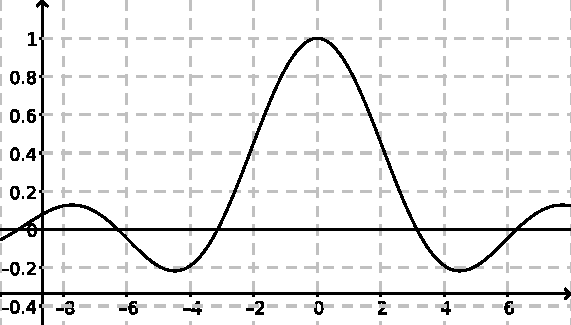
\includegraphics[scale=0.6]{figures/roots-newton4}
\par\end{center}
\begin{enumerate}
\item Metode Newton akan konvergen ke akar yang mana jika $x_{0}=2.5$?
\item Apa yang akan terjadi jika $x_{0}=0$?
\item Tentukan suatu nilai bilangan bulat positif untuk $x_{0}$ yang membuat
metode Newton konvergen ke $2\pi$.
\item Tentukan nilai negatif $x_{0}$, dibulatkan ke persepuluhan terdekat,
yang membuat metode Newton konvergen ke $2\pi$.
\end{enumerate}
\item Gambarkan grafik polinom $p(x)=x^{3}-3x+3$, dan tunjukkan secara
grafis metode Newton untuk $x_{0}=-1$.
\item \octave\ \label{exc:newton-10}Gunakan kode Anda dari soal \ref{enu:secantMethodCode}
untuk mencari sebuah akar fungsi pada interval di soal \ref{enu:bisectionExamples}
\vpageref{enu:bisectionExamples} dengan galat kurang dari $10^{-8}$.
Bandingkan jawaban Anda dengan jawaban dari soal \ref{exc:bisection3}
\vpageref{exc:bisection3}. \hasananswer 
\item \label{exc:newton-11}Jumlah dua bilangan adalah 20. Jika setiap bilangan
dijumlahkan dengan akar kuadratnya, hasil kali kedua jumlah tersebut
adalah $172.2$. Tentukan kedua bilangan itu dengan galat paling besar
$10^{-4}$ dari nilai eksaknya. \hasasolution 
\item \label{exc:newton-12}Berikan contoh situasi ketika metode Newton
gagal pada iterasi kedua (yaitu, $x_{1}$ dapat dihitung tetapi $x_{2}$
tidak dapat dihitung). \hasasolution 
\item Misalkan $h(x)=2.2x^{3}-6.6x^{2}+4.4x$ dan $g(x)=h^{\circ3}(x)$.
Artinya, $g(x)=h(h(h(x)))$. Hampiri salah satu akar $g'(x)$.
\item \label{graph}Untuk nilai-nilai $x_{0}$ mana, secara hampiran, metode
Newton akan konvergen ke $-2.5$?

\begin{center}
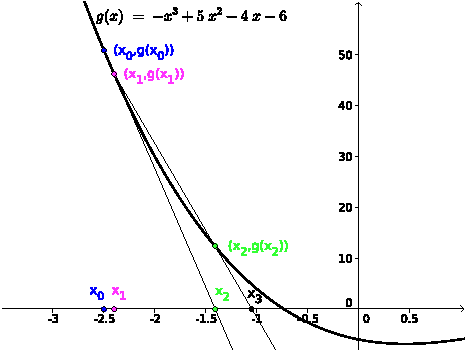
\includegraphics[width=5.5cm]{figures/roots-newton3}
\par\end{center}
\item Untuk fungsi yang ditampilkan pada soal \ref{graph}, tentukan $x_{2}$
dan $x_{3}$ pada metode sekan dengan $x_{0}=-10$ dan $x_{1}=6$.
\item \label{exc:newton-13}Misalkan 
\[
f(x)=10-\int_{0}^{x}\frac{e^{t}}{1+t}\,dt.
\]
Hampiri akar positif $f$. \hasananswer 
\item Dari metode pencarian akar yang telah kita bahas sejauh ini (metode
bagi dua, iterasi titik tetap, metode Newton, metode sekan, dan metode
Steffensen), metode mana yang menurut Anda paling baik? Mengapa?
\end{enumerate}
\noindent\finishexercises

\subsection*{Jawaban}
\begin{description}
\item [{Kekonvergenan~kuadratik?}] \label{que:quadraticConvergence}$\ $

\begin{center}
\begin{tabular}{c|ccc}
$n$ & $x_{n}$ & $\quad$ & $x_{n}$\tabularnewline
\hline 
0 & $2$ &  & $-1$\tabularnewline
1 & $2.5$ &  & $-.7647058823529411$\tabularnewline
2 & $2.666666666666667$ &  & $-.7326286052763475$\tabularnewline
3 & $2.722222222222227$ &  & $-.7320509933083684$\tabularnewline
4 & $2.731741086881274$ &  & $-.7320508075688965$\tabularnewline
5 & $2.732050478023325$ &  & \tabularnewline
6 & $2.732050807568503$ &  & \tabularnewline
$\vdots$ & $\vdots$ &  & $\vdots$\tabularnewline
 & $2.732050807568877$ &  & $-.7320508075688772$\tabularnewline
\end{tabular}
\par\end{center}

Kekonvergenannya tampak kuadratik karena jumlah angka signifikan yang
akurat kurang lebih berlipat dua selama beberapa iterasi terakhir.
\item [{Metode~sekan~secara}] geometris? \label{que:secantMethodGeometrically}
Bandingkan representasi geometris metode sekan berikut dengan representasi
metode Newton (pada halaman \pageref{img:newtonsMethod}). Pada metode
Newton, perpotongan garis singgung dengan sumbu $x$ menentukan iterasi
berikutnya. Pada metode sekan, perpotongan garis sekan dengan sumbu
$x$ menentukan iterasi berikutnya.
\begin{center}
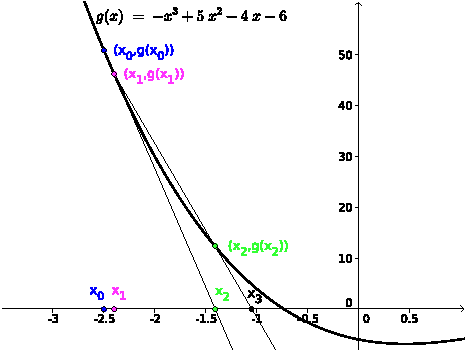
\includegraphics{figures/roots-newton3}
\par\end{center}
\item [{Akar~berikutnya?}] \label{que:nextRoot} Akar berikutnya kira-kira
$2.872257717171606$. Akar ini dapat ditemukan, misalnya, dengan metode
Newton menggunakan $x_{0}=2.81$. Perhatikan bahwa perhitungan ini
sangat peka terhadap kondisi awal karena terdapat begitu banyak akar
yang saling berdekatan. Sebagai contoh, memulai dengan $x_{0}=2.8$
justru menghasilkan akar $9.662623060421268$!
\end{description}

